\section{Digital signalbehandling (DSP)}
\label{DSP}
\index{digital signalbehandling}
\index{digital signal processing (DSP)}
\index{DSP|see {digital signalbehandling}}
\index{Software Defined Radio}
\index{SDR|see {Software Defined Radio}}
\index{FPGA}

\emph{Digital signalbehandling} (eng. \emph{Digital Signal Processing (DSP)})
har blivit allt viktigare i vardagen och så även inom amatörradion i och med
att \emph{Software Defined Radio (SDR)} blivit en viktig del i allt fler
radior och även användning av vanliga datorer.

I grunden så bygger det på att man digitaliserar signalerna, processar det
digitalt i en processor eller programmerbar logikmodul (FPGA), och sedan
omvandlar det till analoga signaler igen.
När man gör detta i mjukvara i en processor kallar man det för SDR\footnote{Software Defined Radio --- det svenska begreppet är \emph{mjukvarudefinierad radio} vilket är en direktöversättning av begreppet på engelska.}.

Har man en dedikerad processor för att göra det kallar man det för en
\emph{Digital Signal Processor (DSP)}.
Processingen kan även göras av dedikerad logik som inte kan programmeras i
normal form som en processor, det är fortfarande
\emph{Digital Signal Processing}, men används nu mer mest för de delarna av
processing där man behöver utföra samma standardiserade jobb fort och effektivt
så att en processor kan utföra de mindre frekventa jobben, men som däremot kan
tillåtas vara mer komplexa.

En GPS-mottagare är ett exempel på en sådan mottagare, där dedikerad hårdvara
hanterar många miljoner samples per sekund, men processar dem till några värden
per millisekund som sedan processas vidare i en processor.

För att kunna förstå detta behöver vi gå igenom grunderna i konvertering av
signalerna mellan analogt och digitalt, och tillbaka.

\subsection{Sampling och kvantisering}
\textbf{HAREC a.\ref{HAREC.a.1.10.1}\label{myHAREC.a.1.10.1}}
\index{sampling}
\index{sample-takt}
\index{sample rate}
\index{sample period}
\index{Sample (S)}
\index{enheter!Sample (S)}
\index{tidsdiskret}
\index{kvantisering}
\index{quantize}
\index{Pulse Code Modulation (PCM)}
\index{PCM}

Analoga signaler är vad vi kallar för kontinuerliga i tid, de varierar spänning
och ström som ett kontinuerligt variation av värdet, så snabbt att vi kan
hantera det fulla radio-spektrat och mer därtill.
Detta fungerar dock inte så väl i den digitala världen.
Dels vill man ha värden i digital form, så vi behöver omvandla våra spänningar
och strömmar till tal, och dels behöver vi göra det i en jämn takt.

\emph{Sampling} (från engelskan) är vad det låter som, vi tar ett prov-värde
(sample) då och då, och i detta sammanhang gör vi det i en jämn takt,
\emph{sample-takten} (eng. \emph{sample rate}.
Denna benämner vi ofta med \(f_S\) och dess \emph{period-tid}
\(T_S=\frac{1}{f_S}\) förekommer också.
Sampeltakten är alltså den jämna takt varmed vi får värden.
Det förekommer lite slarvigt att man benämner den för att vara 1\,MHz, men det
mer korrekta är att man har 1\,MS/s dvs 1 miljon samples per sekund, där S
representerar Samples.

Bild \ref{fig:BildII1-37} illustrerar hur en analog signal samplas och
kvantiseras i en ADC, för att processas i en DSP, för att därefter konverteras
till analog signal med DAC och filtreras.

\begin{figure*}
	\begin{center}
		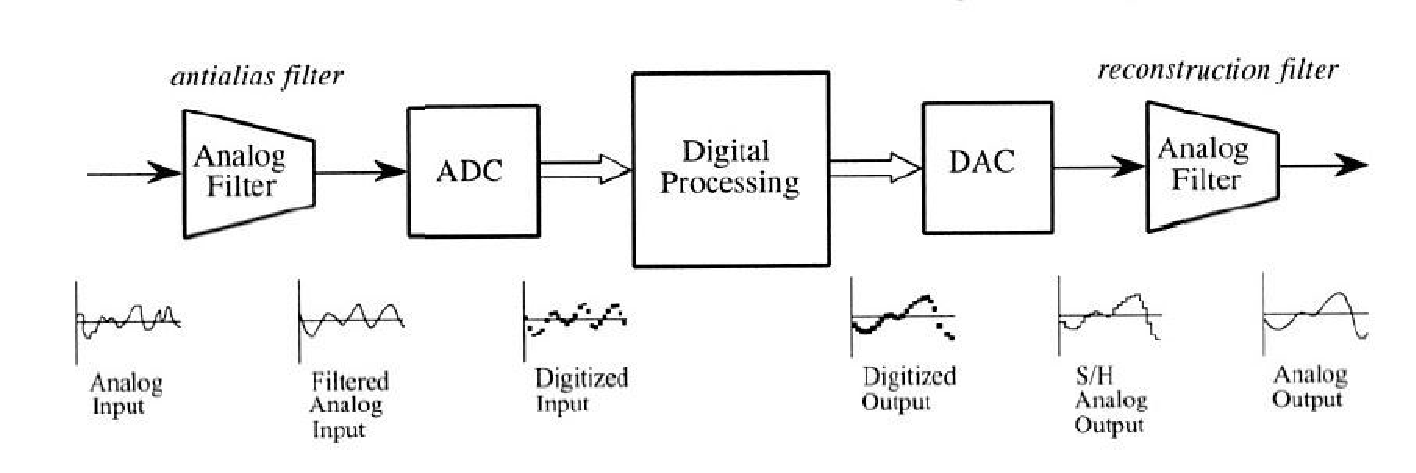
\includegraphics[width=\textwidth]{images/cropped_pdfs/bild_2_1-37.pdf}
		\caption{Sampling med ADC, DSP och DAC för att återvinna analog signal}
		\label{fig:BildII1-37}
	\end{center}
\end{figure*}

Medan sampling är den process som ger oss \emph{tids-diskreta} värden istället
för tids-kontinuerliga värden så är värdena fortfarande inte representerade som
tal, dvs. värdes-diskreta istället för värdes-kontinuerliga.
För att åstadkomma detta behöver man omvandla värdena till fasta värden, en
process som kallas för \emph{kvantisering} (eng. \emph{quantize}).

För att kvantisera värden har man ofta ett fixt avstånd mellan stegen på en
trappstege av värden, varje steg kallas ibland för kvantiserings-steg och
storleken på varje kvantiserings-steg avgör därmed hur hög upplösning man får.
Har man t.ex. ett kvantiserings-steg på 0,1\,V så blir 0 till 0,1\,V tolkat som
0, 0,1--0,2\,V tolkat som 1 osv.
Bild \ref{fig:BildII1-37} visar hur kvantiseringen sker i ADC-steget.

Denna sista del att omvandla de kvantiserade talen till värden kallas
\emph{Pulse Code Modulation (PCM)}, men det ingår i dagligt tal i kvantiserings-
processen idag som en naturlig representation.
Denna omvandling kan göras olinjär, vilket nyttjats i telefoni-system för
kompression, men man har börjat frångå det annat än av kompatibilitetsskäl.

\subsection{Minsta samplingsfrekvensen}
\textbf{HAREC a.\ref{HAREC.a.1.10.2}\label{myHAREC.a.1.10.2}}
\index{nyquistfrekvens}
\index{Nyquist-Shannons samplingsteorem}

\marginnote{
Denna frekvens kallas för nyquistfrekvensen efter Harry Nyquist (1889--1976),
från Stora Kil i Värmland, efter hans banbrytande arbete på Bell laboratories
där han publicerade 1924 och 1928. Det ingår i \emph{Nyquist-Shannons
samplingsteorem} (eng. \emph{Nyquist-Shannon sampling theorem}).
}

Vår nya begreppsvärld har några inneboende begränsningar, en av dem är minsta
samplingsfrekvensen.
Den lägsta frekvensen vi kan hantera i vårt samplade material är fasta värden
(eller DC som man oftast säger) medan den högsta är den när man alternerar
mellan två värden, säg -1 +1 -1 +1 vilket ju ger hälften av samplingstakten
\(f_S\), för perioden för sekvensen blir \(T = 2T_S\) och därmed:
\[
f=\frac{1}{T}=\frac{1}{2T_S}=\frac{f_S}{2}
\]

\subsection{Faltning}
\textbf{HAREC a.\ref{HAREC.a.1.10.3}\label{myHAREC.a.1.10.3}}
\index{faltning}
\index{convolution}
\index{konvolution}
\index{linjär tids-invariant filter}
\index{linear time-invariant filter}
\index{LTI}

Filtrering i den digitala domänen, eller egentligen den tids-diskreta domänen,
kan beskrivas som att filtrets impuls-respons appliceras på signalen, denna
process kallas för \emph{faltning} eller ibland \emph{konvolution} (eng.
\emph{convolution}).
Man kan se det som att varje enskilt sample kommer att spela upp hela filtrets
svängning med sin amplitud, och responsen från alla samples blir därför summan
av alla dessa.
För varje utgående sample så kommer man därför ha summan av filter-responsen
i en viss fördröjning från ett sample som ligger på samma fördröjning bort.

Den matematiskt sinnade kan då använda formeln

\[
	y(n) = \sum_{m=0}^{N-1} x(n-m)h(m)
\]

Där \(x(n)\) är den inkommande sample-strömmen och \(n\) är indexet för det
n:de samplet, \(h(m)\) är filtrets respons och slutligen \(y(n)\) är de utgående
samplen.
Denna summering är densamma som beskrivet ovan och beskriver processen
i tids-planet, dvs. när vi jobbar med tid.

Motsvarande process kan utföras i frekvens-planet, dvs. när vi har konverterat
signalen som amplitud av frekvens istället för amplitud av tid.
Har man då även konverterat filtrets egenskaper så gör man helt enkelt en
multiplikation av signal och filter för varje frekvens:

\[
	Y(f) = X(f)H(f)
\]

Bägge representerar faltning, och är viktig för förståelsen av \emph{linjära
tids-invarianta} filter (eng. \emph{linear time-invariant (LTI)}) filter,
som är det vi i allmänhet fokuserar på.

\subsection{Antivikningsfilter}
\textbf{HAREC a.\ref{HAREC.a.1.10.4}\label{myHAREC.a.1.10.4}}
\index{vikning}
\index{aliasing}
\index{antivikningsfilter}
\index{anti-aliasing filter}

Medan bandbredden vi kan representera är begränsad av Nykvist-frekvensen så
är däremot inte frekvensen det.
Själva samplingen ger upphov till \emph{vikning} (eng. \emph{aliasing}),
sådan att spektrumet efter halva samplings-frekvensen blir vänt så att högre
frekvenser blir lägre.
Denna vikning vänder sedan igen när frekvensen blir den hos
samplings-frekvensen, och spektrumet upprepar sig.
Detta fenomen uppstår alltid när man går mellan tids-kontinuerlig och
tids-diskret tid.

\begin{figure*}
\begin{center}
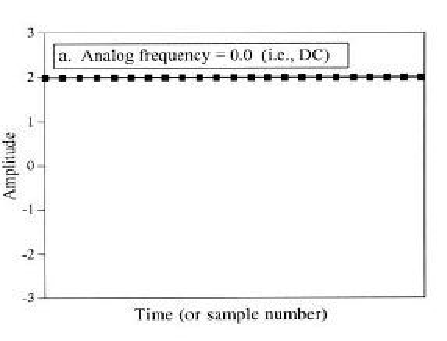
\includegraphics[width=0.45\textwidth]{images/cropped_pdfs/bild_2_1-38.pdf}
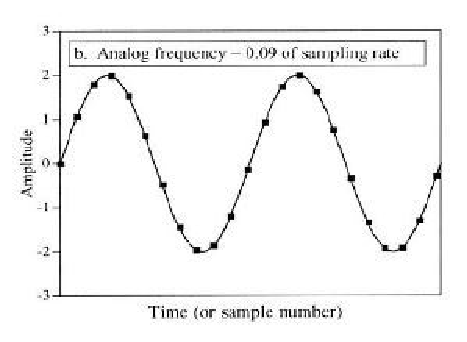
\includegraphics[width=0.45\textwidth]{images/cropped_pdfs/bild_2_1-39.pdf}
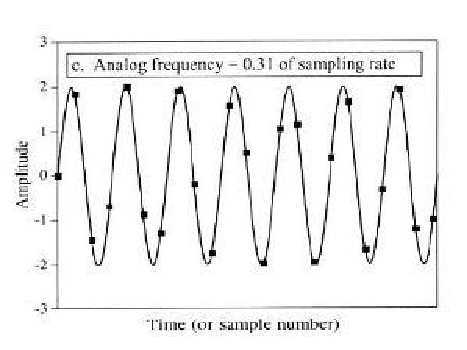
\includegraphics[width=0.45\textwidth]{images/cropped_pdfs/bild_2_1-40.pdf}
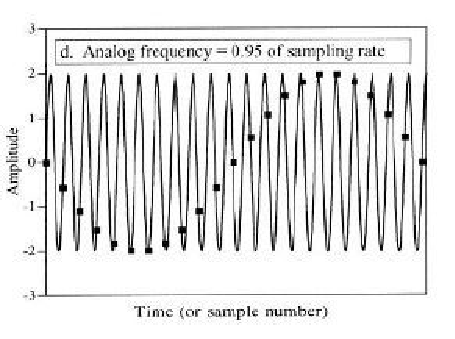
\includegraphics[width=0.45\textwidth]{images/cropped_pdfs/bild_2_1-41.pdf}
\caption{Sampling av DC, 3,6~kHz, 12,4~kHz och 38~kHz med 40~kS/s samplingshastighet}
\label{fig:BildII1-38}
\end{center}
\end{figure*}

Bild \ref{fig:BildII1-38} visar hur fyra olika signaler, DC (likspänning), 
sinus med
3,6\,kHz, 12,4\,kHz och 38\,kHz, samplas med samplingshastigheten 40\,kS/s.
Fallet med DC är uppenbart enkelt, alla punkterna hamnar på samma spänning.
En lågfrekvens sinus, som fallet är med 3,6\,kHz här, får man punkter spridda
över kurvan och de påminner om den ursprungliga sinusen, än mer om man knyter
samman punkterna, vilket anti-aliasingfiltret i praktiken gör.

En frekvens som är nära nykvistfrekvensen, så som 12,4\,kHz in i 40\,kS/s och
dess 20\,kHz nykvistfrekvens, så är sample-punkterna nästa helt alternerande
mellan högsta och lägsta läge. Detta fall är det svårt att se den bakomliggande
sinus-signalen för ett otränat öga, men kan fortfarande rekonstrueras med ett
antialiasingfilter.

Ett ännu svårare fall är 38\,kHz, där punkterna visar en sinus med 2\,kHz, då
frekvensen vikt sig ned run nykvistfrekvensen, och eftersom infrekvensen är
18\,kHz över nykvistfrekvensen hamnar den därför 18~kHz under nykvistfrekvensen,
dvs. på 2\,kHz i det här fallet. Denna vikning är det man försöker undvika med
anti-aliasing-filtret, eftersom toner kan vika sig ned och bli störningar.
Denna vikning sker både vid själva samplingen men även omvänt när man lägger ut
en signal analogt igen. Därför krävs filtrering i bägge riktning.

Vid sampling så kan alltså högre frekvenser vika ned sig i spektrat.
Detta är oftast oönskat, varvid man har ett filter före ingången som
undertrycker oönskade signaler.
För t.ex. tal-signaler använder man ett lågpass filter för att undertrycka de
oönskade signalerna högre upp.
Detta filter kan istället användas för ett visst frekvensband för att
konvertera ned detta band i processen, något som är väldigt populärt i SDR
sammanhang.
I bägge dessa fall är filtret ett \emph{anti-vikningsfilter} (eng.
\emph{anti-aliasing filter}).

Omvänt, när man ska konvertera från tids-diskret till tids-kontinuerlig
signal så viker sig signalen uppåt i frekvens, och för att undertrycka dessa
oönskade frekvenser används på samma sätt ett anti-vikningsfilter.
På samma sätt som förut kan man antingen få de låga frekvenserna som för tal
med ett lågpass-filter eller högre upp i ett band med ett lämpligt
bandpass-filter.

Antivikningsfilter kan många gånger vara relativt branta, för de måste
undertrycka andra delar av spektrat så att de inte blir en störning.

Vid varje fall när man använder en annan frekvens än den lägsta upp till
nykvist-frekvensen får man vara omsorgsfull för att se till att man inte viker
det tänkta bandet.
Ofta kombinerar man därför med en separat mixer för att flytta bandet på ett
behändigt sätt, men det förekommer också att man väljer samplingstakten för att
inte vika bandet.

\subsection{ADC/DAC}
\marginnote{HAREC a.\ref{HAREC.a.1.10.5}\label{myHAREC.a.1.10.5}}
\index{ADC}
\index{DAC}

För att hantera dessa delar använder man analog-till-digital konverterare
(eng. \emph{Analog-Digital Conversion (ADC)}) samt digital-till-analog
konverterare (eng. \emph{Digital-Analog Conversion (DAC)}).
En ADC tar hand om sampling, kvantisering och PCM-kodning medan en DAC
omvandlar PCM-koden till analog spänning.
Ofta behöver man komplettera med analoga filter, men moderna sigma-delta
omvandlare har kraftigt reducerat kraven.

ADC och DAC köper man idag som färdiga integrerade kretsar, inte sällan med
flera kanaler och det finns även dem som har bägge integrerade i samma krets.
Utvecklingen har gjort att man idag kan köpa 24-bitars 48~kS/s ADC och DAC med
dynamiskt område bättre än 100~dB för väldigt låg kostnad.
